%=======================================================================
%  CS-3810 Design Practices in Computer Science -- Assignment 1
%  Project 3: Interactive Data Structure and Algorithms Visualizer
%
%  Sections 3, 4, 5.3 and 6 answer the assignment brief directly.
%  Placeholders written as <LIKE THIS> in red must be replaced by the team.
%  Submission: rename the compiled PDF to  A1_<team_name>.pdf
%=======================================================================
\documentclass[11pt,a4paper]{article}

\usepackage[T1]{fontenc}
\usepackage{lmodern}
\usepackage[margin=2.3cm,top=2.7cm,bottom=2.7cm,headheight=14pt]{geometry}
\usepackage{amsmath,amssymb}
\usepackage{booktabs}
\usepackage{longtable}
\usepackage{array}
\usepackage{enumitem}
\usepackage{xcolor}
\usepackage{tikz}
\usetikzlibrary{arrows.meta,positioning,fit,backgrounds,calc}
\usepackage{listings}
\usepackage{caption}
\usepackage{fancyhdr}
\usepackage{microtype}
\usepackage{parskip}
\usepackage[hidelinks]{hyperref}

%------------------------- typography -------------------------
\setlength{\emergencystretch}{2em}   % avoids minor overfull lines without visible spacing cost

%------------------------- colours -------------------------
\definecolor{reqc}{RGB}{0,102,51}
\definecolor{asmc}{RGB}{176,88,0}
\definecolor{boxc}{RGB}{235,242,250}
\definecolor{statec}{RGB}{232,240,254}
\definecolor{rulec}{RGB}{120,120,120}
\definecolor{codec}{RGB}{245,245,247}

%------------------------- column types -------------------------
\newcolumntype{L}[1]{>{\raggedright\arraybackslash}p{#1}}
\newcolumntype{C}[1]{>{\centering\arraybackslash}p{#1}}

%------------------------- shorthands -------------------------
\newcommand{\R}{\textcolor{reqc}{\textbf{[R]}}}     % stated requirement
\newcommand{\A}{\textcolor{asmc}{\textbf{[A]}}}     % team assumption
\newcommand{\ct}[1]{\texttt{#1}}
\newcommand{\fillme}[1]{\textcolor{red}{\textbf{<\,#1\,>}}}
\newcommand{\lt}{\textless{}}
\newcommand{\gt}{\textgreater{}}
\newcommand{\norm}[1]{\ensuremath{\lvert #1 \rvert}}

%------------------------- code listings -------------------------
\lstdefinestyle{base}{
  basicstyle=\ttfamily\footnotesize,
  columns=fullflexible,
  keepspaces=true,
  breaklines=true,
  breakatwhitespace=false,
  showstringspaces=false,
  frame=single,
  framesep=5pt,
  rulecolor=\color{rulec},
  backgroundcolor=\color{codec},
  xleftmargin=8pt,
  xrightmargin=4pt,
  aboveskip=8pt,
  belowskip=8pt
}
\lstset{style=base}
% algorithmic pseudocode
\lstdefinestyle{pseudo}{style=base,numbers=left,numberstyle=\tiny\color{rulec},numbersep=6pt}
% TypeScript / JSON
\lstdefinestyle{ts}{style=base,numbers=none}

\captionsetup{font=small,labelfont=bf,skip=6pt}
\renewcommand{\arraystretch}{1.12}

%------------------------- headers -------------------------
\pagestyle{fancy}
\fancyhf{}
\fancyhead[L]{\footnotesize CS-3810: Design Practices in Computer Science}
\fancyhead[R]{\footnotesize Assignment 1}
\fancyfoot[C]{\footnotesize\thepage}
\renewcommand{\headrulewidth}{0.3pt}

\begin{document}

%=======================================================================
\begin{center}
  {\large\bfseries Department of Computer Science}\\[2pt]
  {\small Ashoka University}\\[10pt]
  {\LARGE\bfseries CS-3810: Design Practices in Computer Science}\\[6pt]
  {\large\bfseries Assignment 1: Project Specification and Analysis}\\[10pt]
  {\large\bfseries Project 3: Interactive Data Structure and Algorithms Visualizer}
\end{center}

\vspace{2pt}
\begin{center}
\renewcommand{\arraystretch}{1.25}
\begin{tabular}{@{}L{4.2cm}L{10.4cm}@{}}
\toprule
\textbf{Assignment Type} & Group Assignment \\
\textbf{Marks} & 100 \\
\textbf{Submission Format} & PDF generated from \LaTeX \\
\textbf{Submission} & Google Classroom \\
\textbf{Naming Convention} & A1\_\fillme{team\_name}.pdf \\
\bottomrule
\end{tabular}
\end{center}

%-----------------------------------------------------------------------
\section*{Document Status and Reading Guide}
\addcontentsline{toc}{section}{Document Status and Reading Guide}

\noindent\fcolorbox{rulec}{boxc}{%
\begin{minipage}{\dimexpr\linewidth-2\fboxsep-2\fboxrule\relax}
\textbf{Action required by the team before submission.} Everything in this document is
complete except the items below, which the team will fill in:
\begin{itemize}[leftmargin=1.4em,topsep=2pt,itemsep=1pt]
  \item \fillme{Team Name}, \fillme{Team Members}, \fillme{Roll Numbers} and
        \fillme{Repository Link} in the table of Section~2.
  \item Replace Section~2.1 with the team's own wording if the team prefers a
        different framing of the project title, motivation and users.
  \item Rename the compiled PDF to \ct{A1\_\fillme{team\_name}.pdf}.
  \item Delete this box before submitting.
\end{itemize}
\end{minipage}}

\medskip
\noindent\textbf{Conventions used in this document.} Assignment instruction~6 requires a
clear separation between what the brief demands and what the team has decided. We use:
\begin{itemize}[leftmargin=1.4em,topsep=2pt,itemsep=1pt]
  \item \R\ --- a requirement stated or directly implied by the project description.
  \item \A\ --- an assumption, design decision or extension made by our team.
\end{itemize}
\noindent\textbf{Scope.} Section~1 orients the reader, Section~2 records team and project
identification, Section~3 covers requirements analysis, Section~4 the functional
specification, Section~5.3 the project-specific technical analysis, Section~6 the
computational theory, and Section~7 the submission checklist. As instructed, only the
subsection of Section~5 that corresponds to our assigned project (Project~3) is
completed. Appendix~A records the proposed implementation stack, which is engineering
context for the team rather than an answer to a graded question.

\medskip
\noindent\textbf{Reading path for a grader:} \S3.1--\S3.3 (what the system must do),
\S4.1--\S4.3 (how it must behave), \S5.3.1--\S5.3.8 (the algorithmic core),
\S6.1--\S6.4 (theory), \S7 (checklist).

\clearpage

%=======================================================================
\section{Purpose of the Assignment}

This document is the first design-stage deliverable for our project. It converts the
assigned project description into a precise software specification and an initial
technical analysis. Following the brief, it establishes what problem the software solves,
who the intended users are and what they want to accomplish, what the system must do, how
it responds to valid and invalid inputs, which data structures and algorithms are required,
and which computational-theory and operating-system concepts are relevant.

As stated in the brief, this is the design and analysis document only; the implementation
is submitted separately through the prescribed GitHub Classroom repository. Every
functional requirement, error condition and use case in this document is therefore written
so that it can be turned directly into a module, a test, or an acceptance criterion.

%=======================================================================
\section{Project Identification}

\begin{center}
\renewcommand{\arraystretch}{1.3}
\begin{tabular}{@{}L{4.2cm}L{10.4cm}@{}}
\toprule
\textbf{Team Name} & \fillme{team name} \\
\textbf{Team Members} & \fillme{member 1}, \fillme{member 2} \\
\textbf{Roll Numbers} & \fillme{roll number 1}, \fillme{roll number 2} \\
\textbf{Assigned Project} & Project 3: Interactive Data Structure and Algorithms Visualizer \\
\textbf{Repository Link} & \fillme{GitHub Classroom repository URL} \\
\bottomrule
\end{tabular}
\end{center}

\subsection{Assigned Project}

\paragraph{Project title.} Interactive Data Structure and Algorithms Visualizer.

\paragraph{Problem statement.} Introductory data-structures courses teach algorithms
through pseudocode on a whiteboard. A learner can follow a lecture and still be unable to
say what the computer is actually holding in memory at line~6 of an insertion routine. The
gap is not the final answer --- any textbook prints the final tree --- it is the
\emph{process}: which pointer is being followed, what is currently on the stack or in the
queue, which nodes have already been visited, and how many comparisons have been spent so
far. These transient facts are invisible on a whiteboard, laborious to draw by hand, and
impossible to rewind.

\paragraph{Motivation.} Three observations motivate the project.
\begin{enumerate}[leftmargin=1.6em,itemsep=2pt]
  \item \textbf{The result does not teach the method.} Seeing a balanced binary search
        tree after five insertions tells a student nothing about why the tree is balanced,
        or why the same five keys inserted in sorted order produce a linked list.
  \item \textbf{Misconceptions are about process, not outcome.} Common errors --- believing
        that breadth-first search jumps to the nearest node, that recursion ``restarts''
        the function, or that removing the head of a list is the slow part --- are all
        claims about intermediate states, and can only be corrected by showing those
        states.
  \item \textbf{Manual tracing does not scale.} Tracing a traversal through a 30-node graph
        by hand is error-prone, which means the learner practises the wrong habit.
\end{enumerate}

\paragraph{Intended users.} \R\ The brief fixes the project, not the audience; we specify
the audience as follows.
\begin{itemize}[leftmargin=1.6em,itemsep=2pt]
  \item \textbf{Primary --- students in an introductory data-structures course}
        \R\ (for whom the tool is a study aid), typically second-year undergraduates who
        have met the pseudocode in class but not yet built a reliable mental model.
  \item \textbf{Secondary --- instructors and teaching assistants} who want to demonstrate
        an operation live in a lecture or a lab, including deliberate worst-case examples.
  \item \textbf{Tertiary --- self-learners and interview candidates} revising standard
        operations and their complexity.
\end{itemize}

\paragraph{Main goal of the application.} \R\ Provide an interactive, step-controlled
visualiser in which a user can select a data structure, select an operation, supply or
load a dataset, and then watch the operation execute one step at a time --- with the
structural view, the line-by-line algorithm and the auxiliary state (array, stack, queue,
visited set) advancing in lockstep --- together with a plain-English explanation of the
algorithm and its time and space complexity.

\paragraph{Success criterion for the project as a whole.} \A\ A learner who completes a
walkthrough should be able to predict the next step of a fresh instance of the same
operation, and to state why the operation costs what it costs. Correctness of the
visualisation is therefore a prerequisite, not the goal.

%=======================================================================
\section{Requirements Analysis}

\subsection{User Goals}

The brief asks five questions; we answer each directly.

\paragraph{1. Who will use the application?}
The users are the audiences listed in Section~2.1: students (dominant case), instructors
and TAs demonstrating in class, and self-learners revising. All three share one
characteristic that shapes every requirement below: they are \emph{looking at the
algorithm to understand it}, not to obtain a result. A production library that already
computes the correct tree is worthless to them; a tool that shows \emph{how} it got there
is the whole product.

\paragraph{2. What are the primary tasks the user wants to perform?}
\begin{enumerate}[leftmargin=1.6em,itemsep=2pt]
  \item \textbf{Browse} the catalogue of supported data structures from a persistent
        sidebar and see, for each, the operations it supports.
  \item \textbf{Choose an operation} (for example Tree $\rightarrow$ Insert) and read a
        short step-by-step guide describing what will happen before anything runs.
  \item \textbf{Read the algorithm} in plain English once the operation is selected,
        together with its complexity.
  \item \textbf{Supply a dataset} either by loading a curated preset or by typing their
        own values, and have those values checked before use.
  \item \textbf{Control the execution}: play, pause, step forward, step back, restart,
        change speed, and optionally scrub to a particular step.
  \item \textbf{Observe three synchronised views} simultaneously: the structure itself,
        the line-by-line algorithm with the current line highlighted, and the auxiliary
        values (the array being scanned, the stack, the queue, the visited set).
  \item \textbf{Understand the cost} of the operation: theoretical complexity, and the
        number of steps actually consumed by this input.
  \item \textbf{Recover from mistakes}: correct invalid input and re-run, or reset the
        session and start a different structure.
\end{enumerate}

\paragraph{3. What information does the user provide?}
\begin{itemize}[leftmargin=1.6em,itemsep=2pt]
  \item A \textbf{structure selection} and an \textbf{operation selection} (navigation
        only).
  \item A \textbf{dataset}: either the choice of a preset scenario, or a list of values
        typed or pasted into a field. For a graph, an edge list or adjacency list.
  \item An optional \textbf{target value} for operations that need one (search key,
        delete key).
  \item \textbf{Control commands}: play, pause, step forward, step back, restart, speed,
        scrub position.
\end{itemize}

\paragraph{4. What output or feedback should the user receive?}
\begin{itemize}[leftmargin=1.6em,itemsep=2pt]
  \item An \textbf{animated structural view} of the current step, with the element being
        examined distinctly marked and pointers/indices drawn explicitly.
  \item A \textbf{pseudocode panel} in which the line currently executing is highlighted
        and scrolled into view.
  \item An \textbf{auxiliary-state panel} showing exactly the values the algorithm holds
        at this step, with changes since the previous step emphasised.
  \item A one-sentence \textbf{narration} of what the current step is doing, and a
        \textbf{step counter} (``step 7 of 23'').
  \item A \textbf{complexity panel} for the operation, and the observed step count for the
        current run.
  \item \textbf{Input validation feedback} per value, naming the value and the reason it
        was rejected.
  \item \textbf{Error feedback} for invalid inputs and for illegal operations (popping an
        empty stack, deleting an absent key), stated in terms of the algorithm, not as a
        raw exception.
\end{itemize}

\paragraph{5. What would constitute a successful interaction?}
A successful interaction is one in which the user, at the end,
\begin{itemize}[leftmargin=1.6em,itemsep=2pt]
  \item can \textbf{predict} the next step of a fresh instance without running the tool,
  \item can \textbf{explain} the cost of the operation in terms of the input size, and
  \item can \textbf{point} at the intermediate state responsible for a worst case (for
        example the sorted-input binary search tree degenerating to a chain).
\end{itemize}
These are behavioural, and we operationalise them as the usability targets in
Section~4.3 (NFR-U1, NFR-U3) rather than as claims about the animation.

\subsection{Functional Requirements}

Each requirement records the user action or input, the processing the system performs, the
expected output, and the constraints and failure conditions that apply. Requirement
identifiers are referenced from Section~3.3 (errors) and Section~4.2 (use cases).

{\footnotesize
\setlength{\tabcolsep}{3pt}
\begin{longtable}{@{}L{0.9cm}L{2.4cm}L{3.0cm}L{3.6cm}L{2.6cm}L{2.4cm}@{}}
\toprule
\textbf{ID} & \textbf{Functionality} & \textbf{Input / Action} & \textbf{System Processing} &
\textbf{Expected Output} & \textbf{Constraints \& Failure Conditions} \\
\midrule
\endfirsthead
\toprule
\textbf{ID} & \textbf{Functionality} & \textbf{Input / Action} & \textbf{System Processing} &
\textbf{Expected Output} & \textbf{Constraints \& Failure Conditions} \\
\midrule
\endhead
\bottomrule
\endlastfoot

FR1 & Structure catalogue and navigation &
Click a structure (List, Stack, Queue, Tree, Graph) in the persistent sidebar. &
The router resolves the structure route; the description, permitted operations and default
dataset are read from a single static structure catalogue. &
A landing panel for that structure: description, list of supported operations, and
complexity summary. &
\R\ Catalogue is static configuration, so no network call and no failure mode beyond an
unknown route, which redirects to the catalogue. \\

FR2 & Operation menu and guided entry &
Click an operation inside a structure (for example Tree $\rightarrow$ Insert). &
Open the operation workspace and load the step-by-step guide for that
(structure, operation) pair. &
A pop-out guide listing prerequisites and a numbered walkthrough, with \emph{Continue} and
\emph{Skip guide} actions. &
\A\ Guide text is authored per operation. A missing guide falls back to generic text and
logs a content gap; it never blocks execution. \\

FR3 & Algorithm explanation and complexity panel &
None (rendered when the operation is selected); a toggle collapses it. &
Look up the plain-English description, the pseudocode listing, and the best / average /
worst time and space complexity for the operation. &
An explanation panel below the visualiser plus a complexity card. &
\R\ Content must describe the algorithm that is actually traced. Failure: content drift
between prose and code, mitigated by a review checklist and by linking each listing to the
generator module. \\

FR4 & Preset dataset loading &
Select a preset scenario (``balanced BST, 7 keys'', ``sorted input (degenerate)'',
``graph with a cycle''). &
Validate and construct the initial structure from a fixed JSON fixture; clear any previous
trace. &
The structure rendered at step~0, auxiliary panels initialised, preset name shown. &
\A\ Presets are curated fixtures under version control. Failure: a malformed fixture
produces a load error and the previous session is preserved. \\

FR5 & Custom value entry &
Type or paste one or more values, separated by commas, spaces or newlines. &
Tokenise, trim, and classify each token (valid integer, empty, duplicate, out of range);
build a preview of the accepted dataset. &
Per-token status chips and a preview of the dataset that will be used. &
\A\ Limits: at most 200 tokens, integers in $[-9999, 9999]$. Failure: if no token is
accepted, \emph{Visualise} stays disabled with a hint showing a valid example. \\

FR6 & Input validation and rejection of invalid data &
Same input as FR5. &
Validate each token independently against type, range, count and structure-specific rules
(duplicate policy; graph endpoints must exist). &
Inline messages naming the offending token and the reason; rejected tokens are shown but
never forwarded. &
\R\ Validation must be total: every token is reported, not only the first. Failure of the
requirement is defined as the engine ever receiving raw user text. \\

FR7 & Execution trace generation &
Press \emph{Visualise} with a valid request. &
Run the instrumented algorithm as a pure function; append one immutable step object per
meaningful state change; compute a summary. &
An ordered, deterministic array of steps, plus step count, comparison count and conclusion. &
\R\ The engine is free of any UI dependency and is deterministic. Failure: a step-budget
guard truncates pathological traces and reports the truncation. \\

FR8 & Structural visualisation &
Supply a trace and a step index (from playback or scrubbing). &
Compute the render model for the current step (node states, edge states, pointer positions)
and render it as SVG. &
The structure diagram with the active element highlighted and pointers drawn. &
\A\ SVG remains legible up to about 200 nodes, beyond which the view becomes
pan-and-zoom. Failure: a rendering exception is caught by an error boundary that offers a
reset. \\

FR9 & Pseudocode panel with line highlighting &
Change the step index. &
Map \ct{step.codeLine} onto the operation's authored pseudocode listing and scroll it into
view. &
Line-by-line code with the executing line highlighted. &
\R\ The listing is the single authored source of the line map. Failure: a missing mapping
disables the highlight and logs a warning; it must never crash the panel. \\

FR10 & Auxiliary state panel &
Change the step index. &
Extract the auxiliary payload of the step: array contents and indices, stack, queue,
frontier, visited set, recursion frames. &
Live tables of exactly the values held by the algorithm, with changes emphasised. &
\A\ One panel component per auxiliary kind, selected from the step's \ct{aux.kind}.
Failure: an unknown kind degrades to a key--value list. \\

FR11 & Playback control &
Play, pause, step forward, step back, restart, change speed, scrub. &
A single playback controller owns the only timer, advances a clamped step index, and
publishes it to the views. &
Continuous or single-step animation, keyboard shortcuts, and a ``step $i$ of $n$''
counter. &
\R\ One timer owner only; no algorithm work per frame. Failure: bursts of commands are
coalesced because every command is idempotent and the last one wins. \\

FR12 & Graph construction and BFS/DFS &
Enter or load a graph as an edge list, choose a source vertex, and choose BFS or DFS. &
Validate and build an adjacency list; run the instrumented traversal, emitting discover,
enqueue/dequeue (or push/pop), examine-edge and visit events. &
Traversal animation with frontier and visited colouring, a queue-or-stack panel, and the
final visit order. &
\R\ Neighbour order is fixed to make the traversal reproducible. Failure: an unknown
endpoint or self-loop is rejected at load; unreachable vertices are reported as a separate
component rather than silently ignored. \\

FR13 & Session reset and replay &
Press \emph{Restart}, or \emph{New session}. &
Clear trace, auxiliary state and index; optionally re-run the identical request. &
Step~0 of the same operation, or the catalogue view for a new session. &
\A\ Reset is metadata-only, requires no reload, and is idempotent. \\
\end{longtable}
}

\subsection{Error Conditions and Exception Handling}

For each entry we give how the error can occur, how the system detects it, what the user
sees, and whether the operation is cancelled, retried or recovered. ``Recovered'' means
the operation completes and the anomaly is reported as a result of the run rather than as
a failure.

{\footnotesize
\setlength{\tabcolsep}{3pt}
\begin{longtable}{@{}L{0.9cm}L{3.3cm}L{3.0cm}L{5.9cm}L{2.0cm}@{}}
\toprule
\textbf{ID} & \textbf{Error condition} & \textbf{Detection} & \textbf{Handling and feedback} &
\textbf{Outcome} \\
\midrule
\endfirsthead
\toprule
\textbf{ID} & \textbf{Error condition} & \textbf{Detection} & \textbf{Handling and feedback} &
\textbf{Outcome} \\
\midrule
\endhead
\bottomrule
\endlastfoot

ER1 & Non-integer token: \ct{abc}, \ct{4.2}, \ct{1e3}, \ct{--5}, \ct{12.} &
Tokenizer match against \ct{\^{}-?\textbackslash d+\$} after trimming. &
The token is marked in the input with the reason ``not an integer''; the remaining valid
tokens are kept and shown; \emph{Visualise} is disabled while any token is invalid. &
Cancelled for that token; user edits and retries. \\

ER2 & Value outside the supported range, \norm{v} $\gt$ 9999 &
Range check after parsing. &
Message states the permitted range and the offending value; the token is not accepted. &
Cancelled; retry after edit. \\

ER3 & Empty dataset, or every token invalid &
Zero accepted tokens after validation (FR6). &
\emph{Visualise} is disabled and an empty-state hint shows a valid example such as
\ct{50, 30, 70, 20, 40}. No trace is generated. &
Cancelled; retry after edit. \\

ER4 & Duplicate key on insert &
The comparison step finds an equal key before a null child is reached. &
\A\ Policy: duplicates are rejected. The insert step is shown, the duplicate is highlighted
as ``equal --- skipped'', and a non-blocking notice reports it. The rest of the dataset is
inserted normally. &
Recovered; run continues. \\

ER5 & Search or delete target absent &
Traversal reaches a null child, or the trace finishes with the target never matched. &
The search path stays highlighted in a distinct ``examined'' style, and a banner states that
the value is not present. The trace still completes so the full cost of the failed search
is visible. &
Recovered; result reported. \\

ER6 & Stack underflow, or dequeue/pop on an empty structure &
Size is zero when the operation is requested. &
The control is disabled with a tooltip while empty; if the command arrives from the keyboard
it is ignored and an explicit message is shown. No state change occurs. &
Cancelled; no retry. \\

ER7 & Capacity exceeded (overflow on a full stack or queue) &
Size equals capacity, or token count exceeds the structural cap. &
The push or enqueue is refused with a message naming the capacity; the capacity badge is
highlighted, and for the dynamic variant an ``auto-grow'' note explains that the structure
would have resized. &
Cancelled; run continues with the existing contents. \\

ER8 & More tokens than the supported limit &
Token count check before construction (limit 200). &
The batch is refused as a whole with the count and the limit, and a suggestion to split the
input or use a preset. Nothing partial is loaded. &
Cancelled; retry after edit. \\

ER9 & Malformed graph input: unknown endpoint, self-loop, duplicate edge, non-numeric
weight &
Line-by-line validation of the edge list before the graph is built. &
A per-line error list is shown with the offending line and reason; the load is atomic, so
no partial graph replaces the current one. &
Cancelled; retry after edit. \\

ER10 & Unreachable vertex, or a disconnected graph in BFS/DFS &
The frontier empties while some vertices remain undiscovered. &
The reachable set is reported explicitly (``7 of 10 vertices reachable from A''), the
disconnected component is drawn in a muted style, and the user may restart from another
source. &
Recovered; run continues. \\

ER11 & Pathological trace length (step budget exceeded) &
Step counter guard while generating the trace (budget in the tens of thousands of steps). &
Generation stops at the budget, the partial trace is shown, and a warning states that the
trace was truncated with a recommendation to reduce the input size. &
Recovered in part; truncation disclosed. \\

ER12 & Rapid repeated input causing timer contention (repeated play/pause, or replayed
commands) &
Command coalescing inside the playback controller; only one timer may exist. &
Commands are idempotent and the last one wins, so repeated presses cannot start a second
animation loop. &
Recovered; no visible error. \\

ER13 & Render failure inside a panel (SVG or canvas exception) &
React error boundary around each visualisation panel. &
The failing panel is replaced by a fallback with a \emph{Reset visualiser} action; the rest
of the application, including the code panel, stays usable. &
Recovered; the failure is contained. \\
\end{longtable}
}

%=======================================================================
\section{Functional Specification}

\subsection{System Behaviour}

\subsubsection{Layered architecture}

The brief requires that the algorithm logic be separable from the animation and the user
interface. We achieve this by making the algorithm produce a data structure --- a
\emph{trace} --- that the interface merely replays. Nothing about the user interface is
decided inside the algorithm, and nothing about the algorithm is decided inside the
interface. Four layers are involved, and dependencies point one way only.

\begin{figure}[h]
\centering
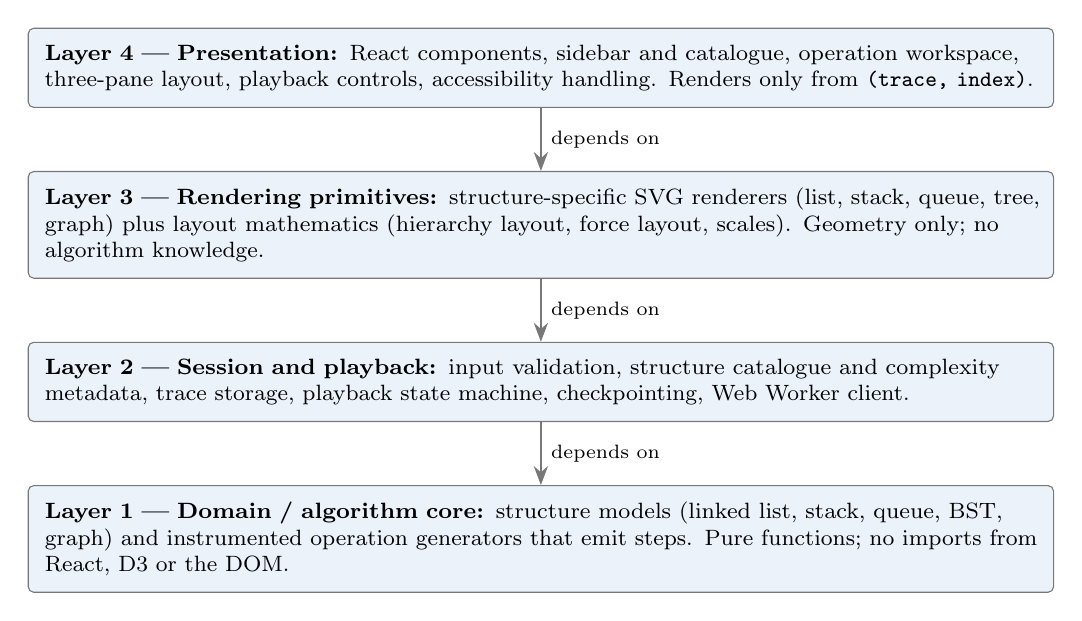
\begin{tikzpicture}[
  font=\footnotesize,
  layer/.style={draw=rulec, rounded corners=2pt, fill=boxc, inner sep=6pt,
                text width=12.6cm, align=left},
  arr/.style={-{Stealth[length=2.4mm]}, draw=rulec, thick}
]
\node[layer] (ui) {\textbf{Layer 4 --- Presentation:} React components, sidebar and
catalogue, operation workspace, three-pane layout, playback controls, accessibility
handling. Renders only from \ct{(trace, index)}.};
\node[layer, below=8mm of ui] (render) {\textbf{Layer 3 --- Rendering primitives:}
structure-specific SVG renderers (list, stack, queue, tree, graph) plus layout mathematics
(hierarchy layout, force layout, scales). Geometry only; no algorithm knowledge.};
\node[layer, below=8mm of render] (session) {\textbf{Layer 2 --- Session and playback:}
input validation, structure catalogue and complexity metadata, trace storage, playback
state machine, checkpointing, Web Worker client.};
\node[layer, below=8mm of session] (core) {\textbf{Layer 1 --- Domain / algorithm core:}
structure models (linked list, stack, queue, BST, graph) and instrumented operation
generators that emit steps. Pure functions; no imports from React, D3 or the DOM.};

\draw[arr] (ui.south) -- node[right,font=\scriptsize,pos=0.5]{depends on} (render.north);
\draw[arr] (render.south) -- node[right,font=\scriptsize,pos=0.5]{depends on} (session.north);
\draw[arr] (session.south) -- node[right,font=\scriptsize,pos=0.5]{depends on} (core.north);
\end{tikzpicture}
\caption{Layered architecture. Imports are permitted only downwards, so Layer~1 can be
executed and tested with no browser present. Layer~2 is the only layer that knows about
time; Layer~4 is the only layer that knows about the DOM.}
\label{fig:layers}
\end{figure}

The rule is enforced mechanically rather than by convention: an import-boundary lint rule
fails the build if Layer~1 imports React, D3 or any module from Layers~3--4.

\subsubsection{The trace: the contract between algorithm and interface}

The central design decision is that an operation is a \emph{generator of states}, not a
mutation of a live object graph. Instrumented operations are written so that every point
at which a learner could ask ``what is happening now?'' emits one step. A step is an
immutable record:

\begin{lstlisting}[style=ts,caption={The step record. Every field is serialisable, which is
what allows the same trace to travel through a Web Worker, be stored in a test fixture, and
be rendered by React.},label={lst:step}]
type Step = {
  index: number;                 // position in the trace, 0-based
  operation: "insert" | "delete" | "search" | "inorder" | "bfs" | ...;
  codeLine: number;              // line of the operation's pseudocode being executed
  narration: string;             // one plain-English sentence for this step
  highlight: {                   // what the viewer should emphasise
    nodes: string[];             // node ids: being compared
    active?: string;             // node id: currently visiting
    edges: string[];             // edge ids: being traversed
  };
  delta: StructureDelta;         // what changed in the structure at this step
  aux: AuxState;                 // array/stack/queue/frontier/visited/recursion
};
\end{lstlisting}

Because a step is immutable and self-describing, the three synchronised views of the user
interface are all pure functions of the same value:
\begin{align*}
\text{structureView} &= f(\text{structure at } i), &
\text{codeView} &= g(\text{step}[i].\text{codeLine}), \\
\text{auxView} &= h(\text{step}[i].\text{aux}). &&
\end{align*}
There is no second source of truth, and no animation state is kept inside the algorithm.

\subsubsection{End-to-end behaviour of a request}

The following is the complete flow from user input to system output, for any operation.

\begin{lstlisting}[style=pseudo,caption={The generic pipeline. Every operation in the
application follows exactly these five stages; only \ct{generateTrace} differs between
operations.},label={lst:pipeline}]
procedure RUN_OPERATION(structure, operation, rawInput, request):
    # Stage 1 -- parse. User text becomes candidate tokens. No side effects.
    tokens   <- tokenise(rawInput)

    # Stage 2 -- validate. Every token is classified; nothing is repaired silently.
    report   <- validate(tokens, structure.rules)   # see the validation listing below
    if report.someRejected and report.accepted is empty:
        return InlineError(report)                        # FR6, ER1-ER3, ER8
    if report.someRejected:
        showWarning(report)                               # run continues, ER4

    # Stage 3 -- build. Construct the initial state of the structure.
    initial  <- buildStructure(structure, report.accepted, request)

    # Stage 4 -- execute. Pure, deterministic, UI-free, optionally in a Web Worker.
    trace    <- generateTrace(initial, operation, request)  # ordered Step[]
    if trace.truncated: showWarning(trace.budget)           # ER11

    # Stage 5 -- present. The interface is now a function of (trace, index).
    controller.load(trace)      # index <- 0, state <- READY
    render(trace, controller.index)
end procedure
\end{lstlisting}

\paragraph{Worked walkthrough (Tree $\rightarrow$ Insert, preset \ct{[50, 30, 70, 45]}).}
This is the flow the user actually experiences, and it is the flow that Section~4.2 turns
into use cases.
\begin{enumerate}[leftmargin=1.6em,itemsep=2pt]
  \item The user clicks \emph{Tree} in the sidebar. Layer~4 reads the tree entry from the
        catalogue and shows its operations (FR1).
  \item The user clicks \emph{Insert}. The guided-entry pop-out appears with the
        step-by-step instructions, and behind it the algorithm explanation and complexity
        card for BST insertion, $O(h)$ time and $O(1)$ auxiliary space (FR2, FR3).
  \item The preset \ct{[50, 30, 70, 45]} is already loaded below the explanation; the user
        may instead type their own values, which are validated token by token (FR4--FR6).
  \item The user presses \emph{Visualise}. Layer~2 asks Layer~1 for a trace. The generator
        walks the insertion loop, emitting one step per comparison, per pointer descent,
        per node creation and per link, in this case approximately 20 steps (FR7).
  \item Layer~2 stores the trace and sets the index to 0. The workspace splits into the
        three panes: the tree, the highlighted pseudocode, and the auxiliary panel showing
        the comparison path and the current key (FR8--FR10).
  \item The user presses \emph{Play}. Layer~2's single timer advances the index; each
        advance repaints all three panes from the immutable step. \emph{Pause},
        \emph{step forward}, \emph{step back} and \emph{Restart} are index operations
        (FR11, FR13).
  \item The run ends at the final step. The narration reports the conclusion, the step
        counter reports the actual cost, and the complexity card reports the theoretical
        one; for the degenerate preset \ct{[10,20,30,40]} the two are visibly different,
        which is the teaching point (FR3, Section~6.4).
\end{enumerate}

\subsubsection{Session state machine}

All user-visible behaviour is governed by one small state machine. No other component may
hold a timer or a mutable step index.

\begin{figure}[h]
\centering
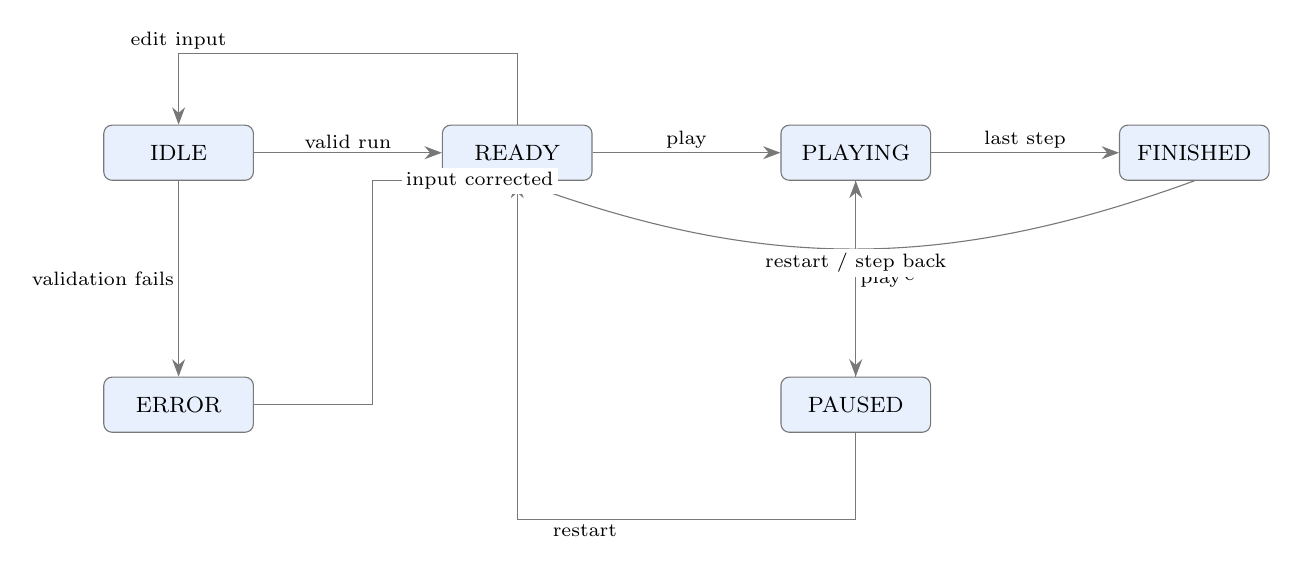
\begin{tikzpicture}[
  font=\footnotesize, >={Stealth[length=2.2mm]},
  state/.style={draw=rulec, rounded corners=3pt, fill=statec, minimum height=7mm,
                minimum width=19mm, align=center},
  err/.style={draw=rulec, rounded corners=3pt, fill=statec, minimum height=7mm,
              align=center},
  e/.style={-{Stealth[length=2.2mm]}, draw=rulec},
  lbl/.style={font=\scriptsize, inner sep=1.5pt, fill=white}
]
\node[state] (idle) at (0,0) {IDLE};
\node[state] (ready) at (4.3,0) {READY};
\node[state] (playing) at (8.6,0) {PLAYING};
\node[state] (done) at (12.9,0) {FINISHED};
\node[state] (paused) at (8.6,-3.2) {PAUSED};
\node[state] (error) at (0,-3.2) {ERROR};

\draw[e] (idle) -- node[lbl,above]{valid run} (ready);
\draw[e] (ready) -- node[lbl,above]{play} (playing);
\draw[e] (playing) -- node[lbl,above]{last step} (done);
\draw[e] (playing) -- node[lbl,right]{pause} (paused);
\draw[e] (paused) -- node[lbl,right]{play} (playing);
\draw[e] (done.south) to[bend left=20] node[lbl,below]{restart / step back} (ready.south);
\draw[e] (paused.south) -- ++(0,-1.1) -| node[lbl,below,pos=0.4]{restart} (ready.south);
\draw[e] (idle) -- node[lbl,left]{validation fails} (error);
\draw[e] (error.east) -- ++(1.5,0) |- node[lbl,right,pos=0.6]{input corrected} (ready.south);
\draw[e] (ready.north) -- ++(0,0.9) -| node[lbl,above,pos=0.5]{edit input} (idle.north);
\end{tikzpicture}
\caption{Session state machine. \ct{PLAYING} is the only state that owns a timer, which is
what makes ER12 impossible by construction rather than by defensive coding. The table below
lists every transition, including the two omitted here for legibility (\ct{FINISHED} to
\ct{IDLE} on a new session, and input editing from \ct{READY}).}
\label{fig:sm}
\end{figure}

\begin{table}[h]
\centering
\small
\begin{tabular}{@{}L{2.1cm}L{3.4cm}L{4.6cm}L{4.9cm}@{}}
\toprule
\textbf{State} & \textbf{Entry condition} & \textbf{Permitted commands} & \textbf{Exit} \\
\midrule
IDLE & Application start, or reset & navigate, select structure, select operation &
Structure and operation both valid $\rightarrow$ READY \\
READY & Trace loaded, index $=0$ & play, step $\pm 1$, restart, edit input, reset &
play $\rightarrow$ PLAYING; edit $\rightarrow$ IDLE \\
PLAYING & Play requested in READY or PAUSED & pause, step, speed, reset &
pause $\rightarrow$ PAUSED; index $= n-1$ $\rightarrow$ FINISHED \\
PAUSED & Pause during playback & play, step $\pm 1$, scrub, restart, reset &
play $\rightarrow$ PLAYING; restart $\rightarrow$ READY \\
FINISHED & Index reached the last step & step back, restart, new session, reset &
restart $\rightarrow$ READY; new session $\rightarrow$ IDLE \\
ERROR & Validation failed, so no trace exists & edit input, reset &
Input corrected and valid $\rightarrow$ READY \\
\bottomrule
\end{tabular}
\caption{State transitions. Because READY, PAUSED and FINISHED all hold a valid trace,
every step control is an array index operation and no state can be lost.}
\label{tab:sm}
\end{table}

\subsubsection{Validation behaviour}

Validation is the only stage that inspects user text, and it is deliberately total: it
classifies every token and never repairs input silently.

\begin{lstlisting}[style=pseudo,caption={The validation pipeline. Rejection is per token,
and the accepted list is the only thing that ever reaches the algorithm.},label={lst:validate}]
procedure VALIDATE(tokens, rules) -> report:
    report <- Report()
    seen   <- empty set
    for each t in tokens:
        if t is empty or whitespace:
            report.reject(t, "empty value");                continue
        if not matches(t, /^-?\d+$/):
            report.reject(t, "not an integer");             continue
        v <- parseInteger(t)
        if |v| > rules.maxAbsValue:
            report.reject(t, "outside range -9999..9999");  continue
        if v in seen and rules.uniqueRequired:
            report.reject(t, "duplicate; duplicates are not inserted"); continue
        if report.accepted.size = rules.maxTokens:
            report.reject(t, "more than 200 values");       continue
        seen.add(v); report.accept(v)
    if report.accepted is empty and tokens is not empty:
        report.fatal("no usable values")
    return report
end procedure
\end{lstlisting}

\subsubsection{Failure containment}

Failures are handled at the layer that can still produce something useful:
validation failures stop the run before any state is created (ER1--ER3, ER8); structural
failures are reported as results of the run (ER4, ER5, ER10); resource failures truncate
and disclose (ER11); and rendering failures are contained by a per-panel error boundary so
that a broken visualiser never takes the explanation or the code panel with it (ER13).

\subsection{Use Cases}

\begin{center}
\small
\setlength{\tabcolsep}{3pt}
\begin{longtable}{@{}L{1.1cm}L{1.7cm}L{7.6cm}L{4.7cm}@{}}
\toprule
\textbf{Use case} & \textbf{Actor} & \textbf{Steps} & \textbf{Expected result} \\
\midrule
\endfirsthead
\toprule
\textbf{Use case} & \textbf{Actor} & \textbf{Steps} & \textbf{Expected result} \\
\midrule
\endhead
\bottomrule
\endlastfoot

UC1 & Student &
1. Open the home page and locate the sidebar. \newline
2. Click \emph{Tree}; read the structure description. \newline
3. Click \emph{Insert}; read the pop-out guide. \newline
4. Press \emph{Continue}. &
The Insert workspace opens with the explanation, complexity card, and preset dataset
visible; nothing has executed yet. (FR1--FR3) \\

UC2 & Student &
1. In Tree $\rightarrow$ Insert, keep the preset \ct{[50, 30, 70, 45]}. \newline
2. Press \emph{Visualise}. \newline
3. Press \emph{Play}, then \emph{Pause} mid-run. \newline
4. Step forward and backward through the comparisons. \newline
5. Press \emph{Restart}, then \emph{Play} to the end. &
The tree, the highlighted pseudocode and the auxiliary panel stay synchronised at every
step; the final tree is a valid BST; the step counter reports the cost of the run.
(FR4, FR7--FR11, FR13) \\

UC3 & Student &
1. In Tree $\rightarrow$ Insert, clear the preset. \newline
2. Type \ct{50, 30, xyz, 70, 30, 99999}. \newline
3. Observe the per-token feedback. \newline
4. Correct the input to \ct{50, 30, 70, 45} and press \emph{Visualise}. &
Each bad token is named with its reason; valid tokens are retained; the run starts only
once the input is clean, and the duplicate never reaches the algorithm.
(FR5, FR6, ER1, ER2, ER4) \\

UC4 & Student &
1. Complete UC2 and stop at the last step. \newline
2. Scrub back to the comparison that decided the left turn. \newline
3. Read the narration and the auxiliary panel for that step. &
The intermediate state of that exact step is reproduced identically, including the
comparison path and the pending link; the run can be resumed from there. (FR10, FR11) \\

UC5 & Student /
Instructor &
1. Choose \emph{Graph}; load the preset with a cycle. \newline
2. Choose BFS and source vertex \ct{A}; press \emph{Visualise}. \newline
3. Watch nodes move from undiscovered to frontier to visited. \newline
4. Repeat with DFS on the same graph. &
The queue or stack panel shows exactly the live frontier; the visit order is displayed and
is reproducible; the DFS and BFS orders differ in the way the theory predicts.
(FR12, Section~5.3.3) \\

UC6 & Student &
1. In Graph, paste an edge list containing \ct{A-B}, \ct{B-B} and \ct{C-Z}. \newline
2. Press \emph{Visualise}. &
Nothing is loaded; a per-line error list explains the self-loop and the unknown endpoint
\ct{Z}; the previously loaded graph is untouched. (ER9) \\

UC7 & Instructor &
1. Load the \emph{sorted input (degenerate)} preset for Tree. \newline
2. Run to completion and compare the height and step count with the balanced preset. &
The two runs produce visibly different structures and step counts, and the complexity card
explains $O(h)$ with $h = n$ for the degenerate case. (FR3, Section~6.4) \\
\end{longtable}
\end{center}

\paragraph{UC2 in detail: inserting into a binary search tree.}
\begin{enumerate}[leftmargin=1.6em,itemsep=2pt]
  \item \textbf{Precondition.} A valid trace exists for \ct{(bst, insert, [50,30,70,45])};
        the session state is READY with index 0.
  \item The user presses \emph{Play}. The controller enters PLAYING and starts its single
        timer at the configured rate.
  \item On each tick the controller increments the index and each of the three panes
        re-renders from \ct{trace[index]}. Step 1 narrates ``start at the root; compare
        50 with 50'', highlighting nothing but the root, with the code panel on the
        comparison line.
  \item The user presses \emph{Pause} on a comparison step. The controller clears the
        timer and enters PAUSED with the index unchanged. The auxiliary panel shows the
        path walked so far and the key being inserted.
  \item \emph{Step forward} and \emph{step back} move the index by $\pm 1$ and cannot leave
        the range $[0, n-1]$; stepping back is exact because the trace is immutable.
  \item \emph{Restart} sets the index to 0 and returns to READY; the trace is not
        recomputed, so the replay is instant and identical.
  \item \textbf{Postcondition.} The final step's structure equals the reference insert
        result, and the step counter reports the comparisons performed.
\end{enumerate}

\paragraph{UC5 in detail: breadth-first search.}
\begin{enumerate}[leftmargin=1.6em,itemsep=2pt]
  \item \textbf{Precondition.} A validated adjacency list with $V$ vertices and a chosen
        source; the traversal is deterministic because neighbour order is the adjacency
        insertion order.
  \item The generator marks the source discovered, enqueues it, and emits a step whose
        auxiliary payload is the current queue contents. Each subsequent step corresponds
        to one dequeue, one examine-edge, or one discover.
  \item Node colouring follows the state of the algorithm, never a decorative choice:
        undiscovered, frontier (queued), current (dequeued and being expanded), and visited
        (finished). Each state also carries a text label so that colour is not the only
        signal (NFR-U2).
  \item If the queue empties with vertices remaining, the run completes and reports the
        reachable set explicitly (ER10).
  \item The final visit order is displayed as a sequence, so the user can compare it with
        the DFS order produced by the same graph.
\end{enumerate}

\subsection{Non-Functional Requirements}

Targets are stated numerically wherever possible. Where a target depends on hardware we
name a reference configuration: a 2020-era laptop with 8~GB of RAM, on the latest stable
Chrome, using the production build.

{\footnotesize
\setlength{\tabcolsep}{3pt}
\begin{longtable}{@{}L{1.3cm}L{2.5cm}L{11.2cm}@{}}
\toprule
\textbf{ID} & \textbf{Category} & \textbf{Requirement and measurable target} \\
\midrule
\endfirsthead
\toprule
\textbf{ID} & \textbf{Category} & \textbf{Requirement and measurable target} \\
\midrule
\endhead
\bottomrule
\endlastfoot

NFR-P1 & Performance & First contentful paint under 2.0~s and time to interactive under
3.0~s on the reference machine, measured with Lighthouse on the production build; initial
JavaScript payload under 500~KB gzipped, which requires importing D3 submodules rather than
the whole bundle. \\
NFR-P2 & Responsiveness & Every control command (play, pause, step, restart) is reflected
on screen within 100~ms. \\
NFR-P3 & Rendering & Animation sustains at least 50~fps (target 60~fps) at $n \le 100$
nodes. This is achievable only because the trace is precomputed: no algorithm work happens
per frame, and a frame is a pure repaint of an immutable step. \\
NFR-P4 & Trace generation latency & For $n \le 200$, a trace is generated in under 200~ms.
Above that, generation runs in a Web Worker so that no main-thread task exceeds 50~ms and
the interface never freezes. \\
NFR-P5 & Memory & Peak trace memory stays under 64~MB for the largest supported input
($n = 200$). A hard step budget (ER11) makes unbounded growth impossible. \\
NFR-C1 & Correctness & Every operation is tested against an independent reference
implementation; the final structure reconstructed from a trace must equal the reference
result for all generated cases, including randomised property-based tests. \\
NFR-C2 & Determinism & The same (structure, operation, dataset) always yields a
byte-identical trace; golden-trace snapshot tests enforce this, and determinism is what
makes UC4 (exact replay of a step) possible. \\
NFR-C3 & Input safety & 100\% of the malformed tokens in the validation test corpus are
rejected with a specific reason. The engine can only be reached by validated values. \\
NFR-C4 & Invariant preservation & Structural invariants (BST ordering, LIFO for stacks,
FIFO for queues, acyclic parent links in trees, no self-loops in graphs) hold at every step
of every trace, asserted in tests. \\
NFR-U1 & Usability & A first-time user completes the UC1 $\rightarrow$ UC2 flow in under
three minutes without external help; target at least 80\% success across five test users. \\
NFR-U2 & Accessibility & WCAG~2.1 AA: text contrast at least 4.5:1; every control reachable
and operable by keyboard (Space to play/pause, left/right arrows to step, R to restart);
step changes announced through an ARIA live region; colour never the sole carrier of
meaning, since each node state also carries a label or shape; \ct{prefers-reduced-motion}
replaces interpolated motion with instantaneous steps. \\
NFR-U3 & Learnability & Every step presents one plain-English narration line, so the user
never has to infer the current action from the animation alone. \\
NFR-S1 & Scalability & Legibility and responsiveness are maintained as inputs grow, with
documented caps: 100 elements for linear structures, 200 nodes for trees and graphs.
Beyond a cap, the view switches to a scrollable or pan-and-zoom mode and states the cap
explicitly rather than degrading silently. \\
NFR-S2 & Extensibility & Adding an operation requires no change to the playback controller
or the interface shell. The acceptance test is that a new operation is added by creating
one generator, one pseudocode listing and one catalogue entry. \\
NFR-M1 & Maintainability & One module per structure and one file per operation; TypeScript
in strict mode; ESLint and Prettier enforced in continuous integration; at least 90\% line
coverage on the algorithm core, with presentational components excluded from that target. \\
NFR-M2 & Modularity & The algorithm core has zero imports from React or any rendering
module. This is enforced by an import-boundary lint rule and a continuous-integration
check, not by convention. \\
NFR-M3 & Testability & Core functions are pure and testable without a DOM; all trace
contract types live in one shared \ct{types} module so that generator and renderer cannot
drift apart. \\
NFR-Po1 & Portability & Runs in the last two versions of Chrome, Edge, Firefox and Safari;
minimum viewport 1280$\times$720; no installation and no backend, deployable as static
files. \\
NFR-Po2 & Responsive layout & The three-pane workspace collapses to a stacked layout below
1024~px and the sidebar collapses to icons below 768~px; the layout must remain usable on a
projector at 1280$\times$720 for classroom demonstration. \\
NFR-Se1 & Security & No \ct{eval} and no execution of user-supplied code; no server
component and no accounts, hence no personal data is stored or transmitted; input length is
capped; user-supplied labels are rendered as text, never as raw markup, which prevents
injection through node labels. \\
NFR-Se2 & Resource safety & Token count, step count and trace size are hard-capped so that
no input can exhaust memory or CPU; the worker is terminated on reset so that no background
computation outlives a session. \\
\end{longtable}
}

%=======================================================================
\section{Project-Specific Technical Analysis}

\noindent The brief asks for the subsection corresponding to the assigned project only. Our
assigned project is Project~3, so subsections 5.1, 5.2 and 5.4 of the brief are deliberately
absent and the numbering below follows the brief exactly.

\setcounter{subsection}{2}   % number this subsection 5.3, as in the brief
\subsection{Project 3: Interactive Data Structure and Algorithms Visualizer}

The project requires interactive visualisation of linked lists, stacks, queues, trees and
graphs, together with step-by-step algorithm execution and complexity information. The
brief lists seven questions; Sections~5.3.1--5.3.7 answer them in order, and Section~5.3.8
answers the closing question about the value of intermediate states. Only Project~3 is
addressed, as instructed.

\subsubsection{Internal representations}

The requirement is to choose, for each structure, a representation that (i) supports the
operations the visualiser must demonstrate, (ii) has a cost model we are willing to display
to a learner, and (iii) can be snapshotted cheaply, because every step must be recorded.

{\footnotesize
\setlength{\tabcolsep}{3pt}
\begin{longtable}{@{}L{1.9cm}L{4.6cm}L{4.3cm}L{4.2cm}@{}}
\toprule
\textbf{Structure} & \textbf{Representation} & \textbf{Why this representation} &
\textbf{Cost shown to the learner} \\
\midrule
\endfirsthead
\toprule
\textbf{Structure} & \textbf{Representation} & \textbf{Why this representation} &
\textbf{Cost shown to the learner} \\
\midrule
\endhead
\bottomrule
\endlastfoot

Linked list & Node objects \ct{\{id, value, next\}} with a \ct{head} reference; pointer
identifiers are stable across steps so that a node can be animated rather than recreated. &
A pointer-based representation is the only one that makes the defining property of a list
--- that order is carried by references, not by position --- visible. An array-backed list
would render index arithmetic and would teach the wrong model. &
Search $O(n)$; insert at head $O(1)$; insert at tail $O(1)$ with a tail pointer, $O(n)$
without; insert at position $k$, $O(k)$; delete $O(n)$ unless the predecessor is known,
which is the distinction the tool is built to show. \\

Stack & Abstract LIFO with \ct{push}, \ct{pop}, \ct{peek}; the visual instance is an
array-backed stack with an explicit \ct{top} index, plus an optional linked-list-backed
variant for the pointer view. &
The array-backed form exposes \ct{top} as a visible index, which is exactly the state a
learner must track; the linked form shows that a stack is an access discipline, not a
layout. Offering both makes the abstraction concrete. &
\ct{push}/\ct{pop}/\ct{peek} amortised $O(1)$ array-backed (with an occasional $O(n)$
resize, which the tool mentions but does not hide); worst-case $O(1)$
linked-list-backed. \\

Queue & Circular buffer: a fixed array plus \ct{head}, \ct{tail} and \ct{count}, with
wraparound indices. &
A circular buffer gives worst-case $O(1)$ enqueue and dequeue and makes FIFO order visible
through the moving indices. The naive ``\ct{array.shift()}'' queue is $O(n)$ per dequeue
and is included deliberately as a comparison preset, because that mistake is common. &
Enqueue $O(1)$; dequeue $O(1)$; \ct{front} $O(1)$; the shift-based variant is shown as
$O(n)$ per dequeue. Space $O(\text{capacity})$. \\

Tree (BST) & Recursive node objects \ct{\{id, value, left, right\}} with an optional
parent reference used only by algorithms that need it, never by the renderer. &
The recursive node is a direct image of the recursive definition of the structure, so the
animation and the definition agree. Keeping parent pointers out of the render model ensures
the drawing shows the tree the algorithms see, not a doubly-linked graph. &
Search, insert, delete $O(h)$ where $h$ is the height: $O(\log n)$ for a balanced tree and
$O(n)$ in the worst case. Traversals $O(n)$. Delete is decomposed into the three standard
cases, each shown separately. \\

Graph & Adjacency list \ct{Map<vertexId, Array<\{to, weight?\}>>} with vertex objects
carrying a value and a layout position; the position is view state and is never read by an
algorithm. &
Demonstration graphs are sparse, and the adjacency list is optimal for exactly the operation
the visualiser performs: iterating a vertex's neighbours. It gives $O(V+E)$ memory and makes
BFS and DFS $O(V+E)$. A sparse matrix would cost $O(V^2)$ memory and make neighbour
iteration $O(V)$ per vertex, hence $O(V^2)$ per traversal. &
Space $O(V+E)$; BFS and DFS time $O(V+E)$; edge existence check is $O(\deg v)$ rather than
$O(1)$, which we state explicitly as the trade-off against a matrix. \\

Trace & Immutable \ct{Step[]} produced by every operation, held by the session layer and
never by a structure model. &
It is the only representation that lets logic and interface be separated, permits exact
step-back, and allows the same run to be asserted in tests. &
Space discussed in Section~5.3.4; rendering is $O(1)$ per step because no algorithm runs
during playback. \\
\end{longtable}
}

\paragraph{The adjacency-matrix alternative.} \A\ We implement the adjacency list as the
default and provide the matrix as an optional comparison view for a small dense graph, since
the trade-off between $O(V+E)$ and $O(V^2)$ is itself part of the curriculum. The matrix is
never used for traversal in the default configuration.

\paragraph{Why not indices into a flat array for every structure?} \A\ A flat array would
make the internal bookkeeping convenient and the animation false. The project's purpose is
to show how references, indices and an abstract access discipline produce the behaviour of
each structure. We therefore choose the representation a textbook would use for each
structure, and accept the slightly larger implementation cost.

\subsubsection{Implementation of insertion, deletion, search and traversal}

Every mutating operation is written as a generator that emits a step whenever the state a
learner must track changes: a comparison, a pointer move, an allocation, a link, a return.
The listing below is the binary search tree insertion generator in the form used by
Layer~1; the \ct{emit} calls are the only difference between this and the plain algorithm.

\begin{lstlisting}[style=pseudo,caption={BST insertion, iterative, instrumented. Emitting a
step at every comparison is what allows the code panel and the auxiliary panel to advance in
lockstep with the tree.},label={lst:bstinsert}]
function generateInsert(root, key) -> Step[]:
    trace <- []; parent <- null; cur <- root
    emit(trace, {codeLine: 1, narration: "Start at the root.", nodes: []})
    while cur is not null:
        emit(trace, {codeLine: 3, narration: "Compare " + key + " with " + cur.value,
                     nodes: [cur.id], active: cur.id})
        parent <- cur
        if key < cur.value:
            emit(trace, {codeLine: 4, narration: key + " < " + cur.value + ": go left."})
            cur <- cur.left
        else if key > cur.value:
            emit(trace, {codeLine: 5, narration: key + " > " + cur.value + ": go right."})
            cur <- cur.right
        else:
            emit(trace, {codeLine: 6, narration: key + " already present: skip."})
            return trace, UNCHANGED          # duplicate policy, ER4

    node <- newNode(key)
    emit(trace, {codeLine: 18, narration: "Reached a null child: create node " + key + ".",
                 delta: {created: [node]}})
    if parent is null:
        root <- node
        emit(trace, {codeLine: 20, narration: key + " becomes the root."})
    else:
        if key < parent.value: parent.left  <- node
        else:                  parent.right <- node
        emit(trace, {codeLine: 26, narration: "Link " + key + " as the child of "
                     + parent.value, edges: [edgeId(parent, node)]})
    return trace, root
end function
\end{lstlisting}

\paragraph{Deletion.} \A\ Deletion is implemented in the three standard cases and each is a
separate visualisation, because the third case (two children) is where learners lose track
of the state: (i) a leaf, unlinked from the parent; (ii) one child, replaced by that child;
(iii) two children, replaced by the in-order successor, which requires the auxiliary panel
to show the successor search separately from the removal. The successor is always taken from
the leftmost node of the right subtree, and the tool states this choice, since taking the
predecessor is equally valid.

\paragraph{Search.} \A\ Search is the insertion loop without the final linking step, so the
code shares the descent routine and both emit identical comparison steps. This sharing is
deliberate: a learner who understands the descent of a search already understands most of an
insert, and the tool makes that visible by highlighting the shared lines.

\paragraph{Traversals.} \A\ In-order, pre-order and post-order are implemented recursively,
because the recursive form is the one taught and the call stack is the state we wish to
visualise. Level-order traversal uses the queue module, so the traversal and the queue
visualisation share one implementation, which guarantees that the picture of the queue is
the queue the algorithm is using. The recursion depth cap described in Section~6.1 protects
against stack overflow on degenerate inputs.

\paragraph{Linear structures.} \A\ Insertion at the head, at the tail, at an arbitrary
position, and deletion by value are each instrumented to emit the pointer moves rather than
only the outcome, since the pointer-move sequence is the material being taught.

\subsubsection{How BFS and DFS are represented and visualised step by step}

Both traversals are implemented over the explicit data structure they are defined by --- a
queue for BFS and a stack for DFS --- so that the auxiliary panel displays the very object
the algorithm is using, rather than a reconstruction of it.

\begin{lstlisting}[style=pseudo,caption={Breadth-first search with instrumentation. The
\ct{aux} payload is the live queue and visited set, which is exactly what the middle and
right-hand panels of the workspace render.},label={lst:bfs}]
function generateBFS(g, source) -> Step[]:
    trace   <- []
    visited <- {source}; queue <- [source]
    order   <- []
    emit(trace, {codeLine: 2, narration: "Enqueue the source " + source,
                 aux: {kind: "queue", values: queue, visited: visited}})
    while queue is not empty:
        v <- dequeue(queue)                       # FIFO: this is what makes it BFS
        order.push(v)
        emit(trace, {codeLine: 4, narration: "Dequeue " + v + " and visit it.",
                     active: v, aux: {kind: "queue", values: queue, visited: visited}})
        for each u in adjacency[v] in insertion order:
            if u not in visited:
                visited.add(u); enqueue(queue, u)
                emit(trace, {codeLine: 6, narration: "Discover " + u + " via " + v,
                             edges: [(v,u)], aux: {kind: "queue", values: queue,
                                                   visited: visited}})
    return trace, order
end function
\end{lstlisting}

DFS is the same listing with \ct{dequeue} replaced by \ct{pop} and the initial container
renamed to a stack. The visual difference the user sees is therefore exactly the difference
the theory predicts: the same graph produces a frontier that grows sideways for BFS and
dives down for DFS. We visualise the recursive form of DFS as well, but as a separate mode,
because in the recursive form the stack is the call stack and must be drawn as a growing
frame column rather than as a data structure the algorithm manipulates.

\paragraph{Node states are algorithm states, not decoration.} The visual palette is
derived from the algorithm's own variables: \emph{undiscovered} (not in the visited set),
\emph{frontier} (in the queue or stack, discovered but not expanded), \emph{current}
(dequeued or popped, being expanded), and \emph{visited} (expansion complete). Because the
palette is a function of the algorithm's variables, a colouring bug is a correctness bug and
is caught by the invariant assertions in NFR-C4. Each state additionally carries a text
label so that the visualisation does not depend on colour alone.

\paragraph{Determinism and honest limitations.} \A\ Neighbours are expanded in adjacency
insertion order, and the tool displays that order, because BFS and DFS are not unique: a
different neighbour order yields a different, equally valid traversal. Stating this is part
of the teaching, not a caveat to hide. In addition, BFS's shortest-path property holds only
for unweighted graphs; the interface labels every graph as unweighted unless the user
supplies weights, and it never claims a shortest path when weights are present.

\subsubsection{How intermediate algorithm states are captured}

This is the central engineering decision of the project, because every other feature ---
step forward, step back, scrubbing, the auxiliary panel, the code highlight, the regression
tests --- is a consequence of it.

\paragraph{Why not simply re-run the algorithm to step 7?} A stateless approach
(\emph{recompute from the start for the requested index}) is simple but makes step-back and
scrubbing cost $O(i)$ per move and, worse, cannot represent nondeterministic or
interaction-dependent state. Since the user will scrub, we need the state to be
\emph{addressable}, not merely reproducible.

\paragraph{The chosen model: an event log with periodic checkpoints.}
\begin{enumerate}[leftmargin=1.6em,itemsep=2pt]
  \item The generator emits a \textbf{delta} per step: what was created, linked, unlinked or
        updated. Deltas are small and constant-sized for all our operations.
  \item The session layer stores the initial state plus the ordered delta log. This log is the
        trace.
  \item Every $k$ steps ($k = 25$ by default) the session layer records a
        \textbf{checkpoint}: a materialised copy of the structure at that index.
  \item To display index $i$, the renderer takes the nearest checkpoint at or before $i$ and
        replays at most $k-1$ deltas. Display cost is therefore $O(k)$, independent of the
        length of the trace.
  \item For small inputs ($n \le 50$) the layer stores full snapshots instead and skips
        checkpointing, because at that size simplicity and exactness are worth more than
        memory.
\end{enumerate}

\paragraph{Space analysis.} Let $s$ be the number of steps and $n$ the input size. Full
snapshotting stores $s$ copies of an $O(n)$ structure, giving $O(ns)$ memory; for a binary
search tree insertion of $n$ keys, $s = \Theta(n \log n)$ in the balanced case, so snapshot
memory is $O(n^2 \log n)$, which is not acceptable at $n = 200$. The delta log stores
$O(1)$ per step, giving $O(s)$ --- approximately 1{,}500 steps of roughly 200 bytes for a
200-key tree, in the order of a few hundred kilobytes --- plus $O(n)$ per checkpoint for
$s/k$ checkpoints. The saving is what makes the 64~MB budget of NFR-P5 comfortable rather
than marginal.

\paragraph{Trace size is bounded.} The step budget of ER11 caps $s$ directly. The largest
supported configurations are 200 elements for linear structures and 200 nodes for trees and
graphs, and the caps are enforced before generation, not after.

\paragraph{The trace as a test artefact.} Because a trace is serialisable and deterministic,
each supported operation has a small golden-trace fixture in the repository. A change in
behaviour appears as a diff of a readable file rather than as a failing screenshot, which is
what makes the algorithm core realistically testable by a two-person team.

\subsubsection{Support for play, pause, restart and step-forward}

All four controls, and scrubbing, are operations on a single integer: the step index.

\begin{lstlisting}[style=pseudo,caption={The playback controller. It owns the only timer in
the application, and every command is a clamped index operation, which is why stepping back
is exact and rapid input cannot start two animations.},label={lst:controller}]
controller:  trace, index, state, speed, timer

procedure load(trace):     self.trace <- trace; self.index <- 0; self.state <- READY
procedure play():          if state = FINISHED: index <- 0
                           state <- PLAYING; startTimer(1000 / (stepsPerSecond * speed))
procedure pause():         stopTimer(); state <- PAUSED
procedure stepForward():   pause(); index <- min(index + 1, trace.length - 1); publish()
procedure stepBack():      pause(); index <- max(index - 1, 0); publish()
procedure restart():       pause(); index <- 0; state <- READY; publish()
procedure seek(i):         pause(); index <- clamp(i, 0, trace.length - 1); publish()
procedure onTick():        if index = trace.length - 1: pause(); state <- FINISHED
                           else: index <- index + 1; publish()
procedure publish():       render(trace, index)   # the only path to the screen
end controller
\end{lstlisting}

\paragraph{Design points.}
\begin{itemize}[leftmargin=1.6em,itemsep=2pt]
  \item \textbf{One timer owner.} Only \ct{PLAYING} may hold a timer. Play is idempotent,
        so a user hammering the play button cannot accumulate intervals (ER12).
  \item \textbf{Timing by accumulated time, not by tick count.} The loop uses
        \ct{requestAnimationFrame} (or a worker timer) and converts elapsed time into whole
        steps, so a slow frame drops steps rather than slowing the logical rate, and the
        speed control means the same thing on every machine.
  \item \textbf{Interpolated transitions are view-only.} Smooth movement between steps is
        produced by the view layer from the two adjacent steps. Disabling motion under
        \ct{prefers-reduced-motion} therefore changes no algorithm behaviour (NFR-U2).
  \item \textbf{Keyboard parity.} Space, arrow keys, \ct{R} and \ct{Home}/\ct{End} map onto
        exactly these commands, so the accessibility path is the same code path as the
        buttons, not a parallel one.
  \item \textbf{The index survives input edits until the trace is replaced}, so a user can
        compare the state at the same step across two datasets, which is how UC7's
        balanced-versus-degenerate comparison is performed.
\end{itemize}

\subsubsection{How complexity information is associated with operations}

Complexity is data, not prose scattered through the interface. Every entry in the structure
catalogue carries a record for each operation:

\begin{lstlisting}[style=ts,caption={Complexity is attached to the catalogue entry that also
drives the operation menu, so the displayed bound cannot disagree with the implemented
operation.},label={lst:complexity}]
type OperationMeta = {
  id: "insert" | "delete" | "search" | "traversal" | ...;
  label: string;                  // shown in the operation menu
  best: string;  average: string; worst: string;   // e.g. "O(log n)", "O(n)"
  space: string;                  // auxiliary space, not total
  assumptions: string[];          // e.g. "h = height; O(log n) requires balance"
  notes?: string;                 // e.g. "amortised", "only for unweighted graphs"
};
\end{lstlisting}

\paragraph{Three properties of this association.}
\begin{enumerate}[leftmargin=1.6em,itemsep=2pt]
  \item \textbf{Provenance.} The same object supplies the menu label, the explanation panel
        and the complexity card, so a bound cannot be attached to the wrong operation, and a
        missing bound is a visible content gap rather than a silent omission.
  \item \textbf{Explicit assumptions.} Bounds whose meaning depends on a variable are stored
        with that variable: tree operations are stated in terms of the height $h$, and the
        card states that $h = O(\log n)$ only when the tree is balanced. Presenting
        $O(\log n)$ for a binary search tree without that qualification would be incorrect,
        and the degenerate preset exists precisely to make the qualification observable.
  \item \textbf{Theory next to observation.} The step counter reports the actual number of
        steps for this input beside the theoretical bound. We use \emph{step count} rather
        than wall-clock time as the observed measure, because step count is
        implementation-independent and therefore comparable to the theory, whereas
        milliseconds are dominated by interpreter effects (Section~6.4).
\end{enumerate}

\paragraph{A limitation we disclose.} \A\ The displayed bounds describe the variants we
implemented, not an ideal library. For example, deleting a node from a singly-linked list
is $O(n)$ because the predecessor must be found; if we later add a doubly-linked variant
with a node reference, the bound becomes $O(1)$, and the card must change accordingly. The
assumptions field exists to keep that distinction honest.

\subsubsection{How algorithm logic is separated from the animation and UI layers}

The separation is the architecture of Figure~\ref{fig:layers}, restated as three enforceable
rules.

\begin{enumerate}[leftmargin=1.6em,itemsep=2pt]
  \item \textbf{The algorithm returns data, not effects.} A generator receives plain values
        and returns a \ct{Step[]}. It never touches the DOM, never imports React or D3, and
        never schedules anything.
  \item \textbf{The interface is a pure function of \ct{(trace, index)}.} Every panel ---
        structure, code, auxiliary, narration, counter --- derives its content from the
        current step. There is exactly one mutable value in the application, the index, and
        exactly one writer of it, the controller.
  \item \textbf{Time lives in one place.} Only the controller knows about timers. Structure
        models have no notion of time; renderers have no notion of sequence.
\end{enumerate}

\paragraph{Enforcement.} \A\ Rules 1 and 2 are checked mechanically: an ESLint
import-boundary rule rejects any import of React, D3 or a rendering module inside the core
directory, and the continuous-integration pipeline runs the core test suite in Node with no
DOM present. If the core suite needs a DOM to pass, the architecture has already been
broken.

\paragraph{Why this separation pays for itself.}
\begin{itemize}[leftmargin=1.6em,itemsep=2pt]
  \item \textbf{Testing.} A trace can be generated and asserted in Node, without a browser,
        without rendering, and without timing. Comparison against a reference implementation
        is a plain function comparison (NFR-C1).
  \item \textbf{Step-back and scrubbing.} They are index arithmetic, not an undone
        animation, because the states already exist.
  \item \textbf{Performance.} All algorithm work happens once, before playback, optionally
        in a worker; the animation loop only repaints.
  \item \textbf{Parallel work for a two-person team.} One member can own the core and its
        tests while the other owns the interface shell and the renderers, with the step
        record as the frozen interface between them.
  \item \textbf{No competing sources of truth.} Visualisation libraries that own the DOM
        while React owns the state produce exactly the class of bug (elements reverting,
        transitions fighting re-renders) that this project cannot afford, since the visual
        state is the graded output. Appendix~A records the resulting rule for D3.
\end{itemize}

\subsubsection{Why showing intermediate states is important for an educational visualiser}

\paragraph{The final state carries almost no information.} Any library can print the correct
tree in microseconds; the answer is the cheapest part of the problem. What a learner lacks is
the \emph{trace}: which comparisons were made, in which order, and what was held in memory
between them. A visualiser that shows only the result is a calculator; a visualiser that
shows the trace is a teacher.

\paragraph{Misconceptions are statements about intermediate states.} ``Breadth-first search
moves to the nearest node'' is a claim about the queue. ``Removing the head of a linked list
is expensive'' is a claim about which pointer must be updated. ``Recursion goes back to the
beginning'' is a claim about the call stack. ``Inserting sorted keys keeps the tree balanced''
is a claim about the height after each insertion. None of these can be corrected by showing
an outcome; all of them are corrected by freezing the relevant step and pointing at the
auxiliary panel.

\paragraph{Process feedback is what changes procedural skill.} Feedback on the correctness
of a final answer tells a learner whether they were right; feedback on the process tells them
where they went wrong. Because the tool makes every intermediate state inspectable and
navigable, a learner can locate the exact step at which their prediction diverged from the
algorithm, which is the moment at which the mental model is repaired.

\paragraph{Predict-then-verify.} Because the controls are step-based, the tool supports a
specific pedagogy that a continuous animation does not: the user states what happens next,
then presses \emph{Step} and finds out. Committing to a prediction before seeing the result
is what converts a passive demonstration into active practice, and it requires exactly the
pause and step-forward capabilities required by the brief.

\paragraph{Reduced cognitive load, and three representations of one state.} Tracing an
algorithm by hand requires holding the structure, the position in the code and the
auxiliary variables in working memory simultaneously. The workspace externalises all three
--- the structure, the highlighted line, and the auxiliary values --- which frees the
learner to reason about the algorithm instead of about bookkeeping. Showing the same state
graphically, textually and symbolically also provides three retrieval routes to the same
idea.

\paragraph{It makes complexity concrete.} The step counter turns an asymptotic claim into an
observation. ``Insertion is $O(h)$'' becomes ``these four keys cost 20 steps and the sorted
preset cost a different number, and here is the step where the tree became a chain''. That
is the bridge from a formula to an understanding, and it is available only if intermediate
states are recorded.

\paragraph{Limitations we accept.} \A\ More intermediate states is not automatically better:
a long trace causes overload and invites step-by-step clicking without thought. We mitigate
this by marking the significant steps (comparison, discovery, link) as distinct from
incidental ones, by giving every step one narration sentence, and by letting the user jump
by significant step rather than by single step.

%=======================================================================
\section{Computational Theory}

Four computational concepts are discussed below. Each is presented as a definition, the
places it occurs in this project, why it is appropriate, and the assumptions or limitations
that come with it. The first two are the concepts our team identified as central; the third
and fourth are included because Section~5.3 requires graph traversal to be visualised step by
step, which cannot be justified without graph theory, and because the project must report
complexity for every operation.

\subsection{Trees and Recursive Traversal}

\paragraph{Definition.} A \emph{tree} is a connected acyclic graph in which one vertex is
distinguished as the root; in a \emph{rooted binary tree} each node has at most two
children, and a \emph{binary search tree} adds the ordering invariant that all keys in the
left subtree are smaller than the node's key and all keys in the right subtree are larger. A
\emph{recursive traversal} is an algorithm defined in terms of itself: a traversal of a tree
consists of doing something at the root and traversing its subtrees. The three depth-first
orders differ only in whether the root is processed before, between or after the two
recursive calls, and \emph{recursion} itself is the technique of solving a problem by
delegating strictly smaller instances of the same problem, with a base case that terminates
the delegation. The state that recursion requires is held implicitly on the call stack.

\paragraph{Where it occurs in the project.} \R\ Trees are one of the five structures the
project must support. Our use of recursion is threefold. First, the tree's own definition is
recursive, so the in-order, pre-order and post-order traversals are implemented recursively
and visualised by showing the growth and unwinding of the recursion frames. Second, the
recursive traversals are drawn against the tree drawn as a recursive structure, so the
correspondence between the code and the picture is immediate. Third, depth-first search on a
graph (Section~6.3) uses the same pattern, and the visualiser presents the recursive and
iterative forms side by side so that a learner sees that the explicit stack of the iterative
form is the call stack of the recursive form.

\paragraph{Why it is appropriate.} The recursive formulation is not merely the shortest
implementation; it is the clearest statement of what the algorithm means. In-order traversal
is ``left subtree, node, right subtree'' and a BST's ordering property is itself recursive,
so a recursive implementation mirrors the structure of the object being processed and is
therefore the least error-prone way to express it. The algebraic identity of the three
traversals --- one implementation, three positions for the visit --- is visible only in the
recursive form, and that identity is precisely what we want to demonstrate. The visualiser
also gains an educational asset: because recursion is invisible in source code, the tool can
show the call stack as a first-class object, which addresses the single most common source of
confusion about recursive algorithms.

\paragraph{Assumptions and limitations.}
\begin{itemize}[leftmargin=1.6em,itemsep=2pt]
  \item Recursion depth is bounded by the height of the tree, so the space cost of a
        recursive traversal is $O(h)$ --- $O(\log n)$ for a balanced tree but $O(n)$ for a
        degenerate one. A traversal of a 200-node chain therefore uses 200 frames.
  \item \A\ JavaScript engines do not guarantee tail-call optimisation, and the call stack is
        finite (in practice a few thousand frames). Degenerate inputs are therefore capped,
        and the core switches to an explicit stack above a depth threshold, with the
        iteration shown in the same visual language as the recursive form.
  \item The recursive traversal silently assumes the structure really is a tree. If a
        malformed parent/child link introduced a cycle, the traversal would not terminate;
        this is why the invariant assertions of NFR-C4 check acyclicity rather than assuming
        it.
  \item Recursion shows the order of visits but hides the arithmetic, so the code panel and
        the narration, not the animation alone, carry the explanation of the base case.
\end{itemize}

\subsection{Stacks and Queues}

\paragraph{Definition.} A \emph{stack} is an abstract data type with last-in-first-out
access: \ct{push} adds an element at the top, \ct{pop} removes the most recently added
element, and \ct{peek} inspects it. A \emph{queue} is the first-in-first-out counterpart:
\ct{enqueue} adds at the rear, \ct{dequeue} removes from the front. Both are \emph{access
disciplines} rather than storage layouts: the same array or linked list can implement either,
and the discipline alone determines the order in which elements come back out. A circular
buffer implements a queue with two indices and a count, so that neither operation needs to
shift elements.

\paragraph{Where it occurs in the project.} \R\ Stacks and queues are two of the five
structures the project must support, so they are the subject of their own modules and
visualisations. Beyond that, they are the machinery of other operations: the queue drives
breadth-first search and level-order traversal, the stack drives depth-first search, the
call stack underlies recursion (Section~6.1), an explicit stack is used for step reversal or
for the iterative forms of the traversals, and the accumulator of the playback loop is a
step queue in the scheduling sense. The auxiliary panel of the workspace exists mainly to
make these containers visible while an unrelated operation runs.

\paragraph{Why it is appropriate.} BFS and DFS are \emph{defined} by FIFO and LIFO
respectively; the only difference between the two traversals is which end of the container
the algorithm takes from. Implementing each traversal with the real abstract data type, and
rendering that same object in the auxiliary panel, means the picture cannot disagree with the
computation. Using a container that merely behaves like a queue (for example, repeatedly
sorting a list, or using an array index shift) would produce the right order while destroying
the very property the visualiser exists to teach, and in the shift case it would also change
the cost from $O(1)$ to $O(n)$ per dequeue --- a mistake we deliberately preserve as a
comparison preset.

\paragraph{Assumptions and limitations.}
\begin{itemize}[leftmargin=1.6em,itemsep=2pt]
  \item An array-backed stack has amortised $O(1)$ \ct{push}, but a resize is $O(n)$ and is
        therefore not constant in the worst case; the complexity card distinguishes
        \emph{worse-case} from \emph{amortised}, and the linked-list-backed variant is
        offered where a strict worst case matters.
  \item A queue implemented with \ct{Array.shift()} is $O(n)$ per dequeue because the
        remaining elements are re-indexed; \A\ our default is a circular buffer with
        \ct{head}, \ct{tail} and \ct{count}, giving $O(1)$ worst case.
  \item A fixed-capacity container can overflow, which is a genuine error condition for the
        user (ER7) and not an internal detail; the dynamic variant is offered so that the
        distinction between overflow and resizing can be demonstrated.
  \item LIFO and FIFO order characterise the container but do not describe its cost: the
        bound depends on the underlying representation, which is why the tool always pairs
        the discipline with its implementation.
\end{itemize}

\subsection{Graphs, Breadth-First Search and Depth-First Search}

\paragraph{Definition.} A \emph{graph} $G = (V, E)$ consists of a set of vertices and a set
of edges, each edge joining two vertices; edges may be directed or undirected and may carry
weights. A graph is commonly stored as an \emph{adjacency list} (for each vertex, the list of
its neighbours) or as an \emph{adjacency matrix} (a $|V| \times |V|$ table). \emph{Breadth-first
search} explores a graph in increasing distance from a source, using a queue as its frontier,
and \emph{depth-first search} explores as far as possible along one branch before retreating,
using a stack (explicit or the call stack). Both classify the edges they traverse into
\emph{tree edges}, which form a spanning tree of the reachable component, and
\emph{non-tree edges}, which are what BFS and DFS reveal about the structure of the graph.

\paragraph{Where it occurs in the project.} \R\ The project requires graphs to be visualised
and BFS and DFS to be represented and visualised step by step (Section~5.3). Our graph module
holds vertices in an adjacency list, and the two traversal generators are the source of the
most demanding animation in the application: discover, enqueue or push, dequeue or pop,
examine an edge, and visit. The frontier and visited sets are displayed live, the examined
edge is highlighted, and the resulting visit order is printed so that two traversals of the
same graph can be compared. Depth-first search is additionally connected to the recursion
discussion, because its recursive form makes the call stack the frontier.

\paragraph{Why it is appropriate.} Graph traversal is the conceptual core of the second half
of an introductory algorithms course, and it is the operation for which step-by-step
visualisation is most valuable, because the state of a traversal --- which vertices are
discovered but not yet expanded --- is almost impossible to hold in mind and is never visible
in the final output. BFS and DFS are also the right choice of \emph{first} graph algorithms
for this project because they are the substrate of nearly everything else: the same
discover/examine machinery, with a priority queue instead of a queue, yields Dijkstra's
algorithm, and with the same frontier machinery becomes a maze solver. Showing them properly
establishes the pattern. The adjacency list is appropriate because demonstration graphs are
sparse, because it gives $O(V+E)$ memory and $O(V+E)$ traversal time, and because iterating
a vertex's neighbours is exactly the unit of work the animation displays.

\paragraph{Assumptions and limitations.}
\begin{itemize}[leftmargin=1.6em,itemsep=2pt]
  \item The $O(V+E)$ traversal bound presumes the adjacency-list representation. With an
        adjacency matrix, listing a vertex's neighbours costs $O(V)$, so a traversal costs
        $O(V^2)$ regardless of how few edges exist. The tool states which representation is
        in use whenever a bound is displayed.
  \item BFS returns shortest paths in the number of \emph{edges}, which is a shortest path in
        terms of \emph{time} only if every edge has the same cost. The interface therefore
        labels every graph as unweighted unless weights are supplied, and never claims a
        minimum-cost path for a weighted graph.
  \item The traversal order is not unique: it depends on the order in which neighbours are
        expanded. \A\ We fix that order to adjacency insertion order and display it, so
        results are reproducible, and we state that other orders are equally correct.
  \item \A\ DFS is implemented iteratively with an explicit stack for large graphs, because
        the recursive form has depth $O(V)$ and could exhaust the call stack; the recursive
        form is retained as a visualisation mode with the same depth cap as Section~6.1.
  \item Two-dimensional layout is not part of the algorithm. Keeping vertex positions in the
        view layer, and out of the graph model, is what prevents a layout change from
        altering the traversal.
\end{itemize}

\subsection{Complexity Analysis and Data Representation}

\paragraph{Definition.} \emph{Complexity analysis} describes how the resources an algorithm
consumes --- time and memory --- grow as a function of its input size, expressed with
asymptotic notation such as $O$, $\Omega$ and $\Theta$, and differentiated into best, average
and worst cases, with \emph{amortised} analysis used where a sequence of cheap operations is
occasionally interrupted by an expensive one. Closely related is \emph{data representation
and abstraction}: the choice of how a value is laid out in memory, and the choice of which
details an interface exposes and which it hides. Representation determines cost, and
abstraction determines what a client is allowed to assume.

\paragraph{Where it occurs in the project.} \R\ The project must associate complexity
information with operations, which appears in three places. First, every operation carries a
bound, its cases and its auxiliary space in the catalogue record of Listing~\ref{lst:complexity}, and that bound
is displayed beside the visualiser. Second, the observed step count of each run is displayed
next to the theoretical bound, which is how the user sees that a degenerate binary search
tree of $n$ keys behaves as a chain. Third, the choice of representation is itself an
exercise in complexity: the adjacency list against the adjacency matrix, the circular buffer
against the shift-based queue, the array-backed stack against the linked-list-backed stack,
and the delta-log trace against full snapshotting are all trade-offs the project makes
explicit.

\paragraph{Why it is appropriate.} Complexity is the reason the structures in this project
exist. If insertion into a search tree were always $O(n)$ there would be no reason to prefer
it to a sorted array; if a stack and a queue had equal access costs there would be no reason
to distinguish them. The visualiser makes the link between structure and cost observable, and
it does so with the measure that belongs to the algorithm rather than to the machine: the
count of the operations that the model charges for. Abstraction is appropriate for the same
reason: the trace record is an abstraction boundary that lets the algorithm core and the
interface evolve separately (Section~5.3.7), and the stack and queue modules reveal only
LIFO and FIFO behaviour, which is what allows one traversal generator to accept either
container.

\paragraph{Assumptions and limitations.}
\begin{itemize}[leftmargin=1.6em,itemsep=2pt]
  \item Asymptotic bounds describe behaviour as $n$ grows; they say nothing about small
        inputs, where constant factors dominate. A linear structure with ten elements may
        convincingly outperform a tree, and the tool does not disguise this.
  \item Bounds are stated for the variant implemented. The costs are worst-case over inputs
        of a given size and assume the model charge (one comparison, one pointer update),
        not the JavaScript engine's actual behaviour.
  \item \A\ For this reason the observed measure is \textbf{step count}, not elapsed time.
        Wall-clock measurements on the same algorithm vary with just-in-time compilation,
        garbage collection and container representation, so times would not be comparable
        between runs or machines; step counts are deterministic and are directly comparable
        with the theoretical bound.
  \item Amortised and worst-case costs must be labelled and never merged: a single
        \ct{push} is $O(1)$ amortised but $O(n)$ in the resizing step, and a complexity card
        that says simply $O(1)$ is incomplete.
  \item Space complexity is reported as \emph{auxiliary} space (the memory used beyond the
        input) unless stated otherwise, because reporting this project's own trace memory as
        the algorithm's space cost would be misleading.
  \item \A\ The 200-node cap, the 200-token cap and the step budget all follow from these
        resource considerations; they are deliberate bounds on the problem size for which the
        visualisation remains honest and legible, not arbitrary limits.
\end{itemize}

%=======================================================================
\section{Submission Checklist}

Every item from the brief is listed below with the section that satisfies it and the
evidence a grader should look for. Items marked \textbf{team action} are the only ones this
document does not complete by itself. Legend: $\boxtimes$ satisfied within this document;
$\square$ awaiting the team's own details (Section~2 and the file name).

{\small
\setlength{\tabcolsep}{4pt}
\begin{longtable}{@{}C{0.7cm}L{6.6cm}L{2.6cm}L{5.2cm}@{}}
\toprule
& \textbf{Checklist item} & \textbf{Where satisfied} & \textbf{Evidence} \\
\midrule
\endfirsthead
\toprule
& \textbf{Checklist item} & \textbf{Where satisfied} & \textbf{Evidence} \\
\midrule
\endhead
\bottomrule
\endlastfoot

$\square$ & Project title and team information are included. &
\S2, \S2.1 & Identification table and the project title, problem statement, motivation,
users and goal. \textbf{Team action:} replace the placeholders in \S2. \\

$\boxtimes$ & User goals are clearly stated. &
\S3.1 & All five questions of the brief answered explicitly, with success defined
behaviourally. \\

$\boxtimes$ & Functional requirements are documented. &
\S3.2 & FR1--FR13, each with input or action, system processing, expected output, and
constraints and failure conditions. \\

$\boxtimes$ & Error conditions and handling are documented. &
\S3.3 & ER1--ER13, each with how it occurs, how it is detected, what the user sees, and
whether the operation is cancelled, retried or recovered. \\

$\boxtimes$ & At least four use cases are provided. &
\S4.2 & Seven use cases (UC1--UC7), with UC2 and UC5 expanded step by step. \\

$\boxtimes$ & Non-functional requirements are discussed. &
\S4.3 & Twenty-one requirements across performance, correctness, usability, accessibility,
scalability, maintainability, modularity, portability, security and resource safety, with
numeric targets. \\

$\boxtimes$ & Project-specific algorithms and data structures are identified. &
\S5.3.1--\S5.3.2 & Representations for all five required structures with justification, and
the instrumented implementations of insertion, deletion, search and traversal. \\

$\boxtimes$ & Computational theory is discussed. &
\S6.1--\S6.4 & Four concepts (trees and recursive traversal, stacks and queues, graphs with
BFS and DFS, complexity analysis and representation), each defined, located in the project,
justified, and bounded by stated assumptions and limitations. \\
\midrule
$\boxtimes$ & The document is compiled successfully using \LaTeX. &
Build & Compiled with the \LaTeX{} engine; the source is submitted as
\ct{A1\_team\_name.tex}. \textbf{Team action:} keep the log free of errors after editing. \\

$\square$ & The PDF follows the required naming convention. &
Title block & \textbf{Team action:} rename the compiled file to
\ct{A1\_\fillme{team\_name}.pdf}. \\

$\square$ & All team members are listed. &
\S2 & \textbf{Team action:} complete the member and roll-number rows. \\
\end{longtable}
}

\paragraph{Additional self-checks the team should run before submitting.}
\begin{itemize}[leftmargin=1.6em,itemsep=2pt]
  \item Read Sections~3.2 and 3.3 against the final code: every requirement should be
        implemented or deliberately deferred, and the document should say which.
  \item Confirm that the complexity claims in \S5.3.6 match the operations that were
        actually implemented (Section~6.4, ``assumptions and limitations'').
  \item Confirm that only Project~3's subsection of Section~5 is present, as the brief
        requires.
  \item Confirm that every \R{} and \A{} marker is still accurate, and that no assumption has
        been presented as a requirement.
\end{itemize}

%=======================================================================
\appendix
\section{Proposed Technology Stack}

This appendix records the implementation stack the team intends to use. It is engineering
context rather than an answer to a graded question, and may be removed without affecting the
answers above.

\paragraph{Fixed constraints.} \R\ The system must be a browser application with an
interactive visualisation, step controls, and no server-side computation; \A\ the team is
working in JavaScript/TypeScript with a shared repository, and the deliverable must be
deployable as static files (NFR-Po1).

{\footnotesize
\setlength{\tabcolsep}{4pt}
\begin{longtable}{@{}L{3.1cm}L{2.9cm}L{8.6cm}@{}}
\toprule
\textbf{Concern} & \textbf{Choice} & \textbf{Justification} \\
\midrule
\endfirsthead
\toprule
\textbf{Concern} & \textbf{Choice} & \textbf{Justification} \\
\midrule
\endhead
\bottomrule
\endlastfoot

Language & TypeScript (strict) &
The trace record of Listing~\ref{lst:step} is the interface between the two members' work. Types make
that interface checkable at compile time and make refactoring the step schema safe, which
matters far more here than the small amount of extra syntax. Plain JavaScript is
workable but trades a one-time cost for a class of runtime bug that is hard to debug in
animation code. \\

Build tooling & Vite &
Fast development server with hot reload, first-class TypeScript and React support, and a
production build that meets the payload target of NFR-P1 without manual optimisation. \\

UI framework & React 19 &
The application is a state machine rendered as a function of \ct{(trace, index)}, which is
the model React is designed for. Declarative rendering also makes the accessibility
requirements of NFR-U2 practical (labels, live regions, focus management) and gives us the
error boundaries used by ER13. \\

Styling & Tailwind CSS &
The layout is a fixed shell --- sidebar, header, three-pane workspace --- with a small,
consistent set of state colours. Utility classes keep that styling local to each component,
which suits a two-person team with no designer, and the state palette can be defined once as
design tokens so that colour is never chosen ad hoc (NFR-U2). It does not replace a
component library: a headless component library for menus, dialogs and tooltips is
recommended for keyboard accessibility. \\

Visualisation library & D3 as a \emph{computation} library, not as a DOM library &
This is the most important stack decision. In a step-based visualiser, React must own the
SVG so that the rendering is a pure function of the current step; if D3 owns the DOM while
React owns the step index, there are two sources of truth, transitions fight re-renders, and
stepping backwards can leave stale elements. We therefore use D3 submodules for geometry and
layout only (\ct{d3-hierarchy} for tree layout, \ct{d3-force} for graph layout,
\ct{d3-scale} and \ct{d3-shape} for coordinates and paths, \ct{d3-interpolate} for view
transitions), and render the elements with React. \ct{d3-selection} is not used for the main
visualisation. \\

State management & A single reducer or a small store (for example Zustand); no algorithm
state in the store &
There is exactly one mutable value, the step index, plus the loaded trace. A reducer or a
minimal store keeps that explicit and keeps the algorithm core out of the UI state. A large
application-wide state library would add indirection without buying anything at this size. \\

Off-main-thread work & Web Worker (NFR-P4) &
Trace generation is pure and serialisable, so it can run in a worker without any change to
the core. This is what keeps the interface responsive for large inputs. \\

Algorithms and tests & Vitest (or Jest) for the core; Playwright or Cypress for one
end-to-end walkthrough &
The core is pure and DOM-free, so unit tests are fast and can be run in Node, which is also
how NFR-M2 is verified. Screenshot-based testing is deliberately avoided because visual
output is expected to change often; golden traces are used instead (NFR-C2). \\

Deployment & Static hosting (GitHub Pages, Netlify or Vercel) &
No backend exists, so deployment is a static build. This also satisfies NFR-Se1: with no
server and no accounts there is no personal data to protect. \\
\end{longtable}
}

\paragraph{Risks in the proposed stack, and the mitigation.}
\begin{itemize}[leftmargin=1.6em,itemsep=2pt]
  \item \textbf{Two rendering paradigms.} The main risk is mixing D3's DOM manipulation with
        React's rendering. \emph{Mitigation:} the rule above is absolute for the main
        visualisation --- D3 computes values, React renders them --- and D3 is permitted to
        own the DOM only inside isolated imperative leaves such as an axis, which never
        contains React children.
  \item \textbf{Transition conflicts.} An animation library that mutates the same attributes
        that React renders will flicker. \emph{Mitigation:} motion is expressed with CSS
        transitions on \ct{transform} and \ct{opacity}, or computed by
        \ct{d3-interpolate} and passed to React as values, never applied to the DOM directly.
  \item \textbf{Timing drift.} \emph{Mitigation:} a single timer owner (Section~5.3.5) drives
        the index from elapsed time rather than counting ticks.
  \item \textbf{Scope size.} Five structures, a catalogue of operations and a three-pane
        workspace is a large surface for two people. \emph{Mitigation:} build one vertical
        slice first
        (linked list, insert, with the three panes and the controller fully working), freeze
        the step contract, then add structures, because NFR-S2 makes each additional
        operation additive rather than invasive.
\end{itemize}

\end{document}
